\documentclass[11pt, a4paper]{article}

%=====================================================================
% PACKAGES
%=====================================================================
\usepackage[top=0.9in, bottom=0.9in, left=0.85in, right=0.85in]{geometry}
\usepackage[utf8]{inputenc}
\usepackage[T1]{fontenc}
\usepackage{lmodern}
\usepackage{xcolor}
\usepackage{colortbl}
\usepackage{graphicx}
\usepackage{tikz}
\usetikzlibrary{arrows.meta, positioning, calc, shapes.geometric, decorations.pathreplacing}
\usepackage{pgfplots}
\pgfplotsset{compat=1.17}
\usepackage{booktabs}
\usepackage{array}
\usepackage{amsmath}
\usepackage{amssymb}
\usepackage{enumitem}
\usepackage{titlesec}
\usepackage{fancyhdr}
\usepackage{caption}
\usepackage{hyperref}
\usepackage{float}

%=====================================================================
% COLORS  (categorical palette: slot1 blue / slot2 orange, status green)
%=====================================================================
\definecolor{accentblue}{HTML}{184F95}
\definecolor{accentblueLight}{HTML}{2A78D6}
\definecolor{accentorange}{HTML}{EB6834}
\definecolor{statusgood}{HTML}{0CA30C}
\definecolor{inkprimary}{HTML}{0B0B0B}
\definecolor{inksecondary}{HTML}{52514E}
\definecolor{inkmuted}{HTML}{898781}
\definecolor{gridline}{HTML}{E1E0D9}
\definecolor{panelbg}{HTML}{F4F7FB}
\definecolor{panelborder}{HTML}{184F95}

%=====================================================================
% HYPERLINKS
%=====================================================================
\hypersetup{
    colorlinks  = true,
    linkcolor   = accentblue,
    urlcolor    = accentblue,
    citecolor   = accentblue,
    pdfauthor   = {Amit Damari, Tomer Zahuri, Tal Franco, Israel Elmaliach},
    pdftitle    = {VLSI ALU Project -- Sklansky Adder -- Group 007}
}

%=====================================================================
% SECTION FORMATTING
%=====================================================================
\titleformat{\section}
  {\normalfont\Large\bfseries\color{accentblue}}
  {\thesection}{0.6em}{}[{\color{accentblue}\titlerule[1.1pt]}]
\titleformat{\subsection}
  {\normalfont\large\bfseries\color{accentblue}}
  {\thesubsection}{0.5em}{}
\titlespacing*{\section}{0pt}{18pt}{8pt}
\titlespacing*{\subsection}{0pt}{12pt}{4pt}

\setlist[itemize]{leftmargin=1.3em, topsep=2pt, itemsep=2pt, parsep=0pt}
\setlist[enumerate]{leftmargin=1.5em, topsep=2pt, itemsep=2pt, parsep=0pt}

%=====================================================================
% HEADER / FOOTER
%=====================================================================
\pagestyle{fancy}
\setlength{\headheight}{22pt}
\fancyhf{}
\renewcommand{\headrulewidth}{0.6pt}
\renewcommand{\headrule}{\hbox to\headwidth{\color{gridline}\leaders\hrule height \headrulewidth\hfill}}
\fancyhead[L]{\small\color{inksecondary} VLSI ALU Project -- Sklansky Adder}
\fancyhead[R]{\small\color{inksecondary} Group 007}
\fancyfoot[C]{\small\color{inkmuted}\thepage}

\captionsetup{font=small, labelfont={bf,color=accentblue}, margin=1em}

%=====================================================================
% HELPERS
%=====================================================================
\newcommand{\sig}[1]{\texttt{#1}}
\newcommand{\fig}[3]{%
\begin{figure}[H]
  \centering
  \includegraphics[width=#2\linewidth]{assets/#1}
  \caption{#3}
\end{figure}}

\graphicspath{{./}}

%=====================================================================
\begin{document}

%=====================================================================
% TITLE PAGE
%=====================================================================
\begin{titlepage}
\newgeometry{top=0in, bottom=0in, left=0in, right=0in}
\centering

\begin{tikzpicture}[remember picture, overlay]
  \fill[accentblue] (current page.north west) rectangle ([yshift=-3.6cm]current page.north east);
  \node[anchor=north, text width=17cm, align=center, yshift=-1.15cm] at (current page.north) {
    {\color{white}\fontsize{34}{40}\selectfont\bfseries VLSI ALU Project}\\[4pt]
    {\color{white!85!accentblue}\Large Part B -- Final Stage \(\cdot\) Group 007}
  };

  \node[anchor=north] at ([yshift=-4.3cm]current page.north) {
    \begin{minipage}{14.5cm}
      \centering
      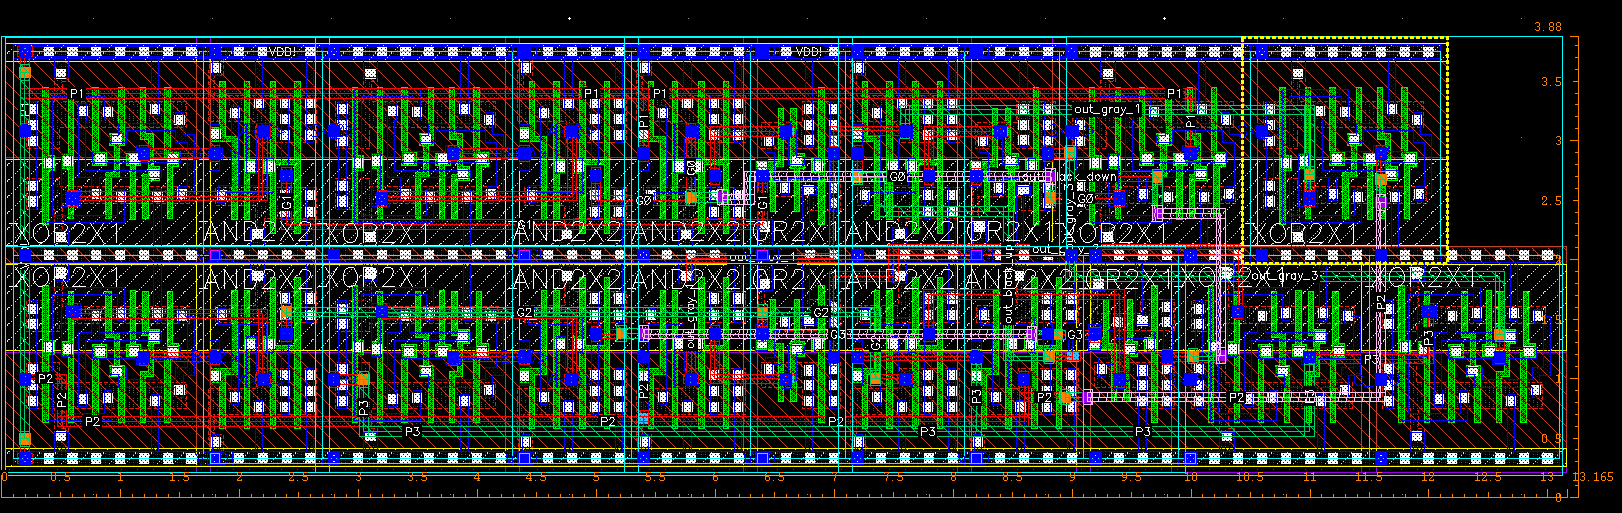
\includegraphics[width=14.5cm]{assets/layout_zoom2.png}
    \end{minipage}
  };
  \node[anchor=north, font=\footnotesize\color{inkmuted}] at ([yshift=-9.1cm]current page.north)
    {Standard-cell layout of the 4-bit Sklansky adder -- Cadence Virtuoso};

  \node[anchor=north, text width=15cm, align=center] at ([yshift=-10.2cm]current page.north) {
    {\Large\bfseries\color{accentblue} A 4-bit ALU Built on a Sklansky Parallel-Prefix Adder}\\[6pt]
    {\normalsize\color{inksecondary} Full-custom schematic capture, physical layout, DRC/LVS
    signoff and post-layout timing characterization in a 45\,nm-class standard-cell
    library, using Cadence Virtuoso and Spectre.}
  };

  \node[anchor=north] at ([yshift=-14.6cm]current page.north) {
    \begin{tikzpicture}
      \draw[accentblue, line width=0.8pt] (0,0) -- (11,0);
    \end{tikzpicture}
  };

  \node[anchor=north, text width=12cm, align=left] at ([yshift=-15.3cm]current page.north) {
    {\small\color{inkmuted}\textbf{SUBMITTED BY}}\\[4pt]
    {\normalsize Amit Damari}\\
    {\normalsize Tomer Zahuri}\\
    {\normalsize Tal Franco}\\
    {\normalsize Israel Elmaliach}
  };

  \fill[accentblue] (current page.south west) rectangle ([yshift=0.5cm]current page.south east);
\end{tikzpicture}

\end{titlepage}
\restoregeometry

%=====================================================================
% EXECUTIVE SUMMARY + RESULTS DASHBOARD
%=====================================================================
\section*{Executive Summary}
\addcontentsline{toc}{section}{Executive Summary}

This report documents the full-custom design of a 4-bit Arithmetic Logic Unit
(ALU) computing $Y = A + B - C$, built around a 4-bit \textbf{Sklansky
parallel-prefix adder} for high-speed addition and a two's-complement
subtractor that reuses the same adder hardware. The design was carried
end-to-end through schematic capture, gate-level sizing, physical layout,
and signoff verification (DRC and LVS, both clean) in Cadence Virtuoso, and
characterized in Spectre across two supply corners (1.2\,V and 0.9\,V) for
setup time, critical-path delay, and maximum clock frequency. A second,
independent exercise (Part 2) explores clock generation with a CMOS ring
oscillator, studying how inverter sizing, RC loading, and output loading
trade off against oscillation frequency.

\medskip
\begin{center}
\begin{tikzpicture}
\node[draw=panelborder, line width=1pt, fill=panelbg, rounded corners=4pt,
      inner sep=12pt, text width=15.4cm] {
\begin{minipage}{15.4cm}
{\bfseries\color{accentblue}\large Results at a Glance}\\[8pt]
\setlength{\tabcolsep}{3pt}
\begin{tabular}{@{}p{7.1cm}@{\hspace{6pt}}p{7.1cm}@{}}
\textcolor{statusgood}{\textbf{\large\checkmark}}\ \textbf{DRC} -- clean, 0 violations &
\textcolor{statusgood}{\textbf{\large\checkmark}}\ \textbf{LVS} -- clean, netlist match \\[10pt]
\textbf{Adder cell area:} 52.29\,\textmu m\textsuperscript{2} (9 AND + 4 OR + 8 XOR) &
\textbf{Layout utilization:} \(\approx\)97.5\% of the raw (unpadded) estimate\\[10pt]
\textbf{f\textsubscript{max} @ 1.2\,V:} \textbf{4.37\,GHz} &
\textbf{f\textsubscript{max} @ 0.9\,V:} \textbf{2.05\,GHz}\\[10pt]
\textbf{Setup time:} \(\approx\)20\,ps @ 1.2\,V / 44\,ps @ 0.9\,V &
\textbf{Rise/fall times:} all signals $<$ 50\,ps at both corners
\end{tabular}
\end{minipage}
};
\end{tikzpicture}
\end{center}

\clearpage
\tableofcontents
\clearpage

%=====================================================================
\section{Introduction}
%=====================================================================

\subsection{Project Library}
The Virtuoso schematic/layout cells for this project are split across two
per-member libraries:

\smallskip
\noindent\textbf{Library owner: \sig{tomerzahuri}}
\begin{itemize}
  \item \sig{4bit\_adder\_pg}, \sig{4bit\_adder\_gray\_cell}, \sig{4bit\_adder\_black\_cell}
  \item \sig{4bit\_register}, \sig{5bit\_register}, \sig{6bit\_register}
  \item \sig{Adder}, \sig{Adder\_tb}, \sig{SUBTRACTOR}, \sig{Subtractor\_tb}
  \item \sig{ALU}, \sig{ALU\_tb}
  \item \sig{Tlogiccq\_meas}, \sig{Tlockq\_sub\_meas}, \sig{Tsetup\_meas}
\end{itemize}

\noindent\textbf{Library owner: \sig{talfranco}} -- Part 2 ring-oscillator cells.

\subsection{Assignment Parameters}
Per the course specification, $X$ is defined as the sum of the last digits
of the student IDs of all group members:
\[
9 + 7 + 7 + 2 = 25
\]
which maps, via the course's assignment table, to $X = 25 \rightarrow Y = 2$.
Variant $Y = 2$ requires implementing an ALU using a \textbf{Sklansky adder},
with the following specification:

\begin{itemize}
  \item \textbf{Logical inputs:} $A[3{:}0]$, $B[3{:}0]$, $C[3{:}0]$, each 4 bits, each latched into its own input register.
  \item \textbf{Output:} a single output $Y[4{:}0]$\footnote{As implemented, the final output register is 6 bits wide (\sig{6bit\_register}) to accommodate the full signed range of $A+B-C$ -- see \S\ref{sec:overview}.}, driven from a register.
  \item \textbf{Encoding:} all values are two's-complement signed integers.
  \item \textbf{Internal register:} the design holds an internal register $X$ where $\langle X \rangle = \langle A \rangle + \langle B \rangle$.
  \item \textbf{Operations:} $\mathrm{ADD}: \langle X \rangle = \langle A \rangle + \langle B \rangle$, \quad $\mathrm{SUB}: \langle Y \rangle = \langle X \rangle - \langle C \rangle$.
  \item \textbf{Supply:} a single nominal $V_{DD} = 1.2\,\mathrm{V}$, referenced to ground.
\end{itemize}

%=====================================================================
\section{ALU Design Overview}
\label{sec:overview}
%=====================================================================

The ALU computes $Y = A + B - C$ from three 4-bit two's-complement inputs,
producing a 6-bit result stored in a register. Figure~\ref{fig:alu-dataflow}
shows the top-level dataflow.

\begin{enumerate}
  \item \textbf{Addition:} $A + B \rightarrow$ latched into a 5-bit register.
        The extra bit absorbs the addition overflow -- e.g.\ the largest
        possible positive sum, $0111_2 + 0111_2 = 1110_2$ (7+7=14), needs
        5 bits to be represented correctly in two's complement.
  \item \textbf{Subtraction:} $(A+B) - C \rightarrow$ latched into a 6-bit
        register, again sized to absorb the result's overflow/sign growth.
  \item \textbf{Overflow handling:} every stage's register is one bit wider
        than the strict minimum, so intermediate results never wrap silently.
\end{enumerate}

\textbf{Key components:}
\begin{itemize}
  \item \textbf{Sklansky adder} -- a parallel-prefix adder used for both the
        addition and (via two's-complement reuse) the subtraction, chosen for
        its logarithmic-depth carry chain.
  \item \textbf{Subtractor} -- built from the same adder, using two's-complement
        inversion of the subtrahend (see \S\ref{sec:impl-adder-sub}).
  \item \textbf{Registers} -- every register is built from per-bit D flip-flops,
        clocked synchronously.
\end{itemize}

\begin{figure}[H]
\centering
\begin{tikzpicture}[
  node distance=6mm and 10mm,
  reg/.style={draw=accentblue, fill=panelbg, rounded corners=2pt, minimum width=1.5cm, minimum height=0.8cm, font=\footnotesize},
  op/.style={draw=accentblue, fill=accentblue!12, rounded corners=2pt, minimum width=1.1cm, minimum height=1.1cm, font=\bfseries\large\color{accentblue}},
  lbl/.style={font=\scriptsize\color{inksecondary}},
  ->, >=Latex, thick, accentblue
]
\node[reg] (Areg) {\sig{A} reg};
\node[reg, below=of Areg] (Breg) {\sig{B} reg};
\node[reg, below=of Breg] (Creg) {\sig{C} reg};

\node[op, right=of Areg, yshift=-4mm] (add) {$+$};
\node[reg, right=16mm of add, yshift=-4mm] (Xreg) {\sig{X} reg};
\node[op, right=14mm of Xreg] (sub) {$-$};
\node[reg, right=16mm of sub] (Yreg) {\sig{Y} reg};

\draw (Areg) -- (add);
\draw (Breg) -| (add);
\draw (add) -- node[lbl, above]{5} (Xreg);
\draw (Xreg) -- node[lbl, above]{5} (sub);
\draw (Creg) -| (sub);
\draw (sub) -- node[lbl, above]{6} (Yreg);
\draw (Yreg) -- ++(1.1,0) node[right, font=\bfseries\color{inkprimary}]{$Y$};

\node[lbl, left=1mm of Areg] {$A[3{:}0]$};
\node[lbl, left=1mm of Breg] {$B[3{:}0]$};
\node[lbl, left=1mm of Creg] {$C[3{:}0]$};
\end{tikzpicture}
\caption{ALU top-level dataflow: $A$ and $B$ are latched and added by the
Sklansky adder into a 5-bit register $X$; $C$ is latched and subtracted from
$X$ by the reused adder/subtractor, producing the final 6-bit result $Y$.
(Redrawn for clarity; the original schematic capture is Figure~\ref{fig:alu-top-schematic}.)}
\label{fig:alu-dataflow}
\end{figure}

%=====================================================================
\section{Sklansky Adder: Theory}
%=====================================================================

\subsection{Core Structure}
The Sklansky adder is a \textbf{parallel prefix tree} that computes every
carry $C_i$ in logarithmic time, rather than rippling a carry bit-by-bit
through the whole word as a naive ripple-carry adder does. It is built from
three logic cells:

\begin{itemize}
  \item \textbf{PG cell} -- generates, per bit, the \emph{propagate} signal
        $P_i = A_i \oplus B_i$ and the \emph{generate} signal $G_i = A_i \cdot B_i$.
  \item \textbf{Black cell} -- combines two adjacent $(G,P)$ group signals into one:
        \[
          G_{\mathrm{group}} = G_{\mathrm{left}} + \left(P_{\mathrm{left}} \cdot G_{\mathrm{right}}\right),
          \qquad
          P_{\mathrm{group}} = P_{\mathrm{left}} \cdot P_{\mathrm{right}}
        \]
  \item \textbf{Gray cell} -- an optimized black cell that only produces the
        group \emph{generate} signal $G_{\mathrm{group}}$, omitting the group
        propagate output where it will never be needed downstream. This
        trims area and wiring in the stages where only the final carry is required.
\end{itemize}

\noindent\textbf{Carry recurrence:} \(\displaystyle C_{i+1} = G_i + P_i \cdot C_i\)
\quad ($C_i$ is the carry \emph{into} bit $i$; $C_0$ is the adder's carry-in, tied to 0 here.)

\noindent\textbf{Final sum:} \(\displaystyle S_i = P_i \oplus C_i\)
\quad (using the same index $i$ as the recurrence above -- e.g.\ $S_1 = P_1 \oplus C_1 = P_1 \oplus G_0$, matching $G_0$ wiring directly into the $S_1$ XOR with no combining cell in Figure~\ref{fig:adder-schematic}, and $S_2 = P_2 \oplus C_2 = P_2 \oplus \text{\sig{out\_gray\_1}}$ one stage later.)

\subsection{Why Sklansky}
\begin{itemize}
  \item \textbf{Speed:} $O(\log n)$ carry-propagation delay, versus $O(n)$ for a ripple-carry adder.
  \item \textbf{Area efficiency:} fewer wires than a Kogge-Stone adder, at the cost of slightly more fan-out per stage; still faster than a Brent-Kung adder for a given cell count.
  \item \textbf{Scalability:} a good fit for the 4-bit width used here, where the logarithmic-depth tree is only two levels deep.
\end{itemize}

\begin{figure}[H]
\centering
\begin{tikzpicture}[
  pg/.style={draw=accentblue, fill=accentblue!10, rounded corners=2pt, minimum width=1.1cm, minimum height=0.7cm, font=\scriptsize},
  gr/.style={draw=accentorange, fill=accentorange!12, rounded corners=2pt, minimum width=1.1cm, minimum height=0.7cm, font=\scriptsize},
  bk/.style={draw=inkprimary, fill=inkmuted!18, rounded corners=2pt, minimum width=1.1cm, minimum height=0.7cm, font=\scriptsize},
  wire/.style={accentblue, line width=0.7pt},
  siglabel/.style={font=\scriptsize, color=inksecondary, fill=white, inner sep=1pt},
  stagelabel/.style={font=\scriptsize\bfseries, color=inkmuted, anchor=east},
  ->, >=Latex
]
% ---- row labels ----
\node[stagelabel] at (-1.1, 0)    {Bit level};
\node[stagelabel] at (-1.1, -2.2) {Stage 1};
\node[stagelabel] at (-1.1, -6.6) {Stage 2};

% ---- leaves ----
\foreach \i/\x in {0/0, 1/3, 2/6, 3/9} {
  \node[pg] (pg\i) at (\x, 0) {PG\i};
  \node[font=\scriptsize\color{inksecondary}] at (\x, 0.62) {$A_\i,B_\i$};
}

% C1 = G0 directly -- no combining cell needed, it's a leaf output
\draw[wire, dashed] (pg0.south) -- ++(0,-1.1);
\node[font=\scriptsize\bfseries\color{accentblue}] at (0, -1.5) {$C_1=G_0$};
\node[font=\scriptsize\color{inkmuted}] at (0, -1.85) {(no cell needed)};

% ---- Stage 1 ----
\node[gr] (l1a) at (1.5, -2.2) {Gray}; % G[0:1]
\node[bk] (l1b) at (7.5, -2.2) {Black}; % (P,G)[2:3]
\draw[wire] (pg0) -- (l1a) node[siglabel, pos=0.55, above] {$G_0$};
\draw[wire] (pg1) -- (l1a) node[siglabel, pos=0.4, above] {$P_1,G_1$};
\draw[wire] (pg2) -- (l1b) node[siglabel, pos=0.4, above] {$P_2,G_2$};
\draw[wire] (pg3) -- (l1b) node[siglabel, pos=0.55, above] {$P_3,G_3$};

% C2 = G[0:1] -- tap off the level-1 Gray cell, dropped low enough to clear
% both the "Stage 1" row label and the continuing bus below
\draw[wire, dashed] (l1a.south west) -- ++(-0.55,-0.5);
\node[font=\scriptsize\bfseries\color{accentblue}, anchor=north east] at ($(l1a.south west)+(-0.6,-0.55)$) {$C_2=G_{0:1}$};

% ---- Stage 2 (pushed well below the bus row so every turn has clear room) ----
\node[gr] (l2a) at (4.5, -6.6) {Gray}; % G[0:2]: combines G[0:1] with PG2
\node[gr] (l2b) at (7.5, -6.6) {Gray}; % G[0:3]=Cout: combines G[0:1] with (P,G)[2:3]

% Fan-out bus: G[0:1] leaves Stage 1 and feeds BOTH Stage-2 cells -- strictly
% orthogonal (horizontal bus, then a plain vertical drop into each cell), with
% a junction dot at the branch and a small hop where it crosses PG2's own
% wire below (the hop marks "crosses, does not connect").
\coordinate (busJ) at (1.5, -4.2);
\draw[wire] (l1a.south) -- (busJ);
\fill[accentblue] (busJ) circle (1.3pt);
\draw[wire] (busJ) -- (4.5,-4.2) -- (l2a.north);
\draw[wire] (busJ) -- (4.5,-4.2) -- (5.7,-4.2) arc (180:0:0.18) -- (6.7,-4.2) -- (6.7,-6.6) -- (l2b.west);
\node[siglabel] at (3, -4.2) {$G_{0:1}$};
\node[siglabel, anchor=east] at (6.6, -5.4) {$G_{0:1}$};

% PG2's second tap (its first tap already went to the Black cell above) --
% enters l2a from the side (east), so it never approaches from above and
% cannot cross paths with the G[0:1] bus dropping into l2a's top.
\draw[wire] (pg2.south) -- (6,-6.6) -- (l2a.east);
\node[siglabel] at (6.4,-3.4) {$P_2,G_2$};

% Black's tap enters l2b straight from above (they share an x-coordinate --
% no jog needed), leaving the west side free for the G[0:1] bus above, so
% neither wire has to bend at the last moment right at the node.
\draw[wire] (l1b) -- (l2b.north) node[siglabel, pos=0.4, right] {$P_{2:3},G_{2:3}$};

\node[font=\scriptsize\bfseries\color{accentblue}] at (4.5,-7.55) {$C_3=G_{0:2}$};
\node[font=\scriptsize\bfseries\color{accentblue}] at (7.5,-7.55) {$C_4=C_{OUT}$};
\draw[wire, dashed] (l2a.south) -- ++(0,-0.55);
\draw[wire, dashed] (l2b.south) -- ++(0,-0.55);
\end{tikzpicture}
\caption{4-bit Sklansky prefix tree, with the exact carry each stage
produces (verified against the group's own gate-level netlist,
Figure~\ref{fig:adder-schematic}) and every wire labeled with the signal it
carries. $C_1{=}G_0$ needs no combining cell at all (bit 0's generate
signal \emph{is} the carry into bit 1); $C_2{=}G_{0:1}$ comes from a single
Gray cell; $C_3$ and $C_4$ (the final carry-out) each need a second stage,
so the tree's worst-case depth is 2 -- consistent with
$\lceil\log_2(4)\rceil=2$. The two wires labeled $G_{0:1}$ leaving the
Stage-1 Gray cell are the same signal fanning out to both Stage-2 cells --
that fan-out is what keeps the tree logarithmic-depth rather than linear.
(Conceptual redraw; the group's actual gate-level netlist is in
\S\ref{sec:impl-adder-sub} and Figure~\ref{fig:floorplan-gatelevel}.)}
\label{fig:sklansky-tree}
\end{figure}

%=====================================================================
\section{Floor Plan and Area Budget}
\label{sec:floorplan}
%=====================================================================

\fig{floorplan_gatelevel}{0.85}{Cell-level floor plan of the 4-bit Sklansky
adder: two rows of PG cells feed a row of Gray/Black cells, which feed the
final XOR row that produces the sum bits.\label{fig:floorplan-gatelevel}}

\textbf{Gate-level implementation:}
\begin{itemize}
  \item 4 $\times$ PG cell -- each built from 1 AND gate + 1 XOR gate.
  \item 3 $\times$ Gray cell -- each built from 1 AND gate + 1 OR gate.
  \item 1 $\times$ Black cell -- built from 2 AND gates + 1 OR gate.
  \item 4 $\times$ XOR gate -- final sum-bit computation.
\end{itemize}

\begin{table}[H]
\centering
\begin{tabular}{@{}lccc@{}}
\toprule
\rowcolor{accentblue!10}
\textbf{Cell} & \textbf{Count} & \textbf{Area (\textmu m\textsuperscript{2})} & \textbf{Total (\textmu m\textsuperscript{2})} \\
\midrule
AND & 9 & 2.128 & 19.152 \\
OR  & 4 & 1.748 & 6.992 \\
XOR & 8 & 3.268 & 26.144 \\
\midrule
\textbf{Total} & \textbf{21} & -- & \textbf{52.288} \\
\bottomrule
\end{tabular}
\caption{Adder gate-count and area budget (9 AND from 4 PG + 3 Gray + 2 Black; 4 OR from 3 Gray + 1 Black; 8 XOR from 4 PG + 4 final-sum).}
\end{table}

\begin{figure}[H]
\centering
\begin{tikzpicture}[font=\small]
  % Proportional stacked bar: widths scaled directly from the area table
  % (12cm total <-> 52.288 um^2, so 1cm = 4.357 um^2)
  \def\wAND{4.395} \def\wOR{1.605} \def\wXOR{6.0}
  \fill[accentblueLight] (0,0) rectangle ++(\wAND,0.9);
  \fill[accentblue]      (\wAND,0) rectangle ++(\wOR,0.9);
  \fill[accentorange]    (\wAND+\wOR,0) rectangle ++(\wXOR,0.9);
  \draw[white, line width=1pt] (\wAND,0) -- ++(0,0.9);
  \draw[white, line width=1pt] (\wAND+\wOR,0) -- ++(0,0.9);
  \draw[inkmuted] (0,0) rectangle (12,0.9);
  \node[color=white, font=\bfseries\small] at (\wAND/2,0.45) {AND -- 19.15\,\textmu m\textsuperscript{2} (37\%)};
  \node[color=white, font=\bfseries\scriptsize, rotate=90] at (\wAND+\wOR/2,0.45) {OR};
  \node[color=white, font=\bfseries\small] at (\wAND+\wOR+\wXOR/2,0.45) {XOR -- 26.14\,\textmu m\textsuperscript{2} (50\%)};
  \node[font=\scriptsize, color=inksecondary, anchor=north] at (\wAND+\wOR/2,-0.15) {OR: 6.99\,\textmu m\textsuperscript{2} (13\%)};
\end{tikzpicture}
\caption{Gate-area budget as a proportion of the total 52.288\,\textmu
m\textsuperscript{2}: XOR gates (needed for every PG cell \emph{and} every
final sum bit) dominate at half the area, despite AND contributing more
individual gate instances (9 vs.\ 8).}
\label{fig:area-breakdown}
\end{figure}

The raw gate-level area sums to \textbf{52.288\,\textmu m\textsuperscript{2}}.
The initial planning estimate padded this by an additional $\sim$20\% (to
$\approx$62.75\,\textmu m\textsuperscript{2}) to account for routing between
blocks. Once the layout was completed, the measured utilized area came in
below even the raw, unpadded estimate -- \textbf{$\approx$97.5\%
($\approx$50.96\,\textmu m\textsuperscript{2})} of the raw gate-level sum,
or $\approx$81\% of the padded planning estimate -- because several VSS
power rails ended up shared between adjacent blocks rather than duplicated
per block.

%=====================================================================
\section{Circuit Implementation}
\label{sec:impl-adder-sub}
%=====================================================================

\subsection{Top-Level ALU}
The ALU is composed of the input/output registers, the adder, and the
subtractor, connected as in Figure~\ref{fig:alu-dataflow}.

\fig{alu_top_schematic}{0.95}{Top-level ALU schematic capture: $A$, $B$, $C$
registers feed the adder and subtractor blocks, producing the final
registered output $Y$.\label{fig:alu-top-schematic}}

To implement the addition, the adder uses the Sklansky algorithm described
in \S3, chosen specifically to reduce the carry-propagation delay compared
to a ripple-carry design.

\subsection{Adder}
\fig{adder_schematic}{0.98}{4-bit Sklansky adder netlist: four \sig{4bit\_adder\_pg}
cells generate per-bit $(P,G)$, which feed a tree of \sig{4bit\_adder\_gray\_cell}
and \sig{4bit\_adder\_black\_Cell} instances, terminating in the final-sum
XOR row.\label{fig:adder-schematic}}

\subsection{Subtractor}
\fig{subtractor_schematic}{0.98}{Subtractor netlist: each bit of the
subtrahend is inverted before entering the same adder structure, with the
carry-in tied high to complete the two's-complement negation
(+1).\label{fig:subtractor-schematic}}

The subtractor is a clean example of hardware reuse: it performs
$X - C$ using the \emph{exact same} adder structure as the addition stage.
Two's-complement subtraction is implemented by inverting every bit of $C$
and feeding the inverted value, together with $X$, into the adder -- the
adder's carry-in supplies the ``$+1$'' that completes the negation.

\begin{figure}[H]
\centering
\begin{tikzpicture}[
  reg/.style={draw=accentblue, fill=panelbg, rounded corners=2pt, minimum width=1.5cm, minimum height=0.8cm, font=\footnotesize},
  inv/.style={draw=accentorange, fill=accentorange!12, rounded corners=2pt, minimum width=2.0cm, minimum height=0.8cm, font=\footnotesize},
  op/.style={draw=accentblue, fill=accentblue!12, rounded corners=2pt, minimum width=1.1cm, minimum height=1.8cm, font=\bfseries\large\color{accentblue}},
  lbl/.style={font=\scriptsize\color{inksecondary}},
  ->, >=Latex, thick, accentblue
]
\node[reg] (Xreg) at (0,0) {\sig{X} reg};
\node[reg] (Creg) at (0,-3) {\sig{C} reg};
\node[inv] (inv) at (3.3,-3) {invert (XOR 1)};
\node[op] (add) at (6,-1.5) {$+$};
\node[reg] (Yreg) at (8.8,-1.5) {\sig{Y} reg};

\draw (Xreg) -- node[lbl, above, pos=0.6]{5} (add.north west);
\draw (Creg) -- node[lbl, above]{4} (inv);
\draw (inv.east) -| node[lbl, pos=0.25, above]{$\overline{C}$} (add.south);
\node[font=\scriptsize\bfseries\color{accentorange}] at (7.1,-2.55) {$C_{in}=1$};
\draw (add) -- node[lbl, above]{6} (Yreg);
\draw (Yreg) -- ++(1.1,0) node[right, font=\bfseries\color{inkprimary}]{$Y$};

\node[lbl, left=1mm of Xreg] {$X[4{:}0]$};
\node[lbl, left=1mm of Creg] {$C[3{:}0]$};
\end{tikzpicture}
\caption{The subtraction trick: $C$'s bits are inverted (a bank of XOR-with-1
gates -- cheaper than a true negation circuit) and fed into the
\emph{same} adder hardware used for $A+B$, with the carry-in tied high to
supply the ``$+1$'' that completes two's-complement negation. The result is
$X + \overline{C} + 1 = X - C$, with zero extra adder logic.}
\label{fig:subtractor-reuse}
\end{figure}

Because the operands are constrained to a signed 4-bit range, this can
overflow: the result becomes too large or too small to represent in the
target bit width. Overflow is detected by comparing the carry into the
most-significant bit against the carry out of it -- if the two differ, the
result is invalid. Equivalently, overflow has occurred whenever two
positive operands sum to a negative result, or two negative operands sum to
a positive one; either case flips the expected sign and signals that the
result cannot be trusted.

\subsection{Standard Cells}
\label{sec:cells}

\begin{figure}[H]
\centering
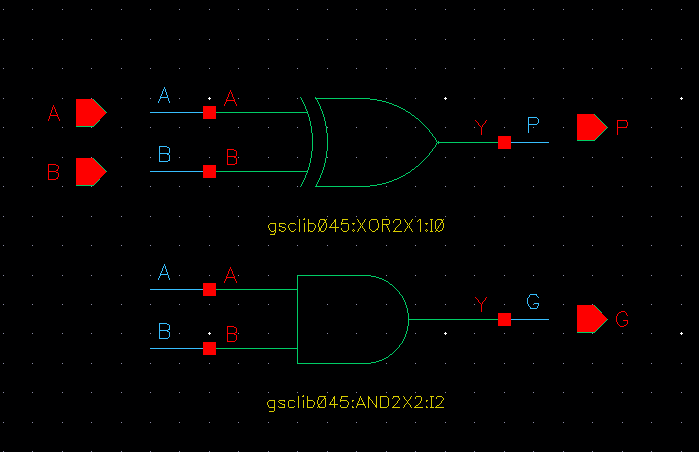
\includegraphics[width=0.72\linewidth]{assets/pg_cell.png}
\caption{PG cell: $P = A \oplus B$ (top, XOR2X1), $G = A \cdot B$ (bottom, AND2X2).}
\end{figure}

\begin{figure}[H]
\centering
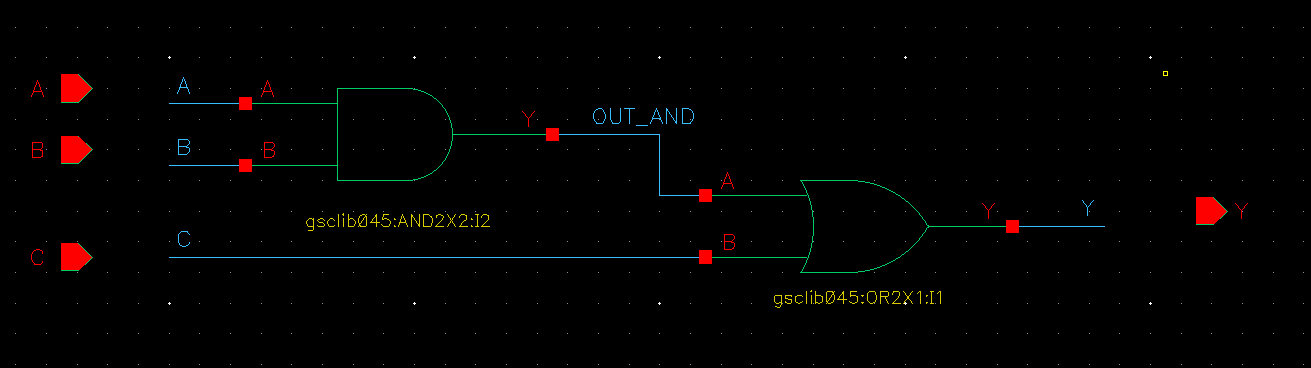
\includegraphics[width=0.72\linewidth]{assets/gray_cell.png}
\caption{Gray cell: computes $G_{\mathrm{group}} = (A \cdot B) + C$ -- i.e.\
$G_{\mathrm{group}} = G_{\mathrm{left}} + (P_{\mathrm{left}} \cdot G_{\mathrm{right}})$
from AND2X2 + OR2X1, omitting the group-propagate output.}
\end{figure}

\begin{figure}[H]
\centering
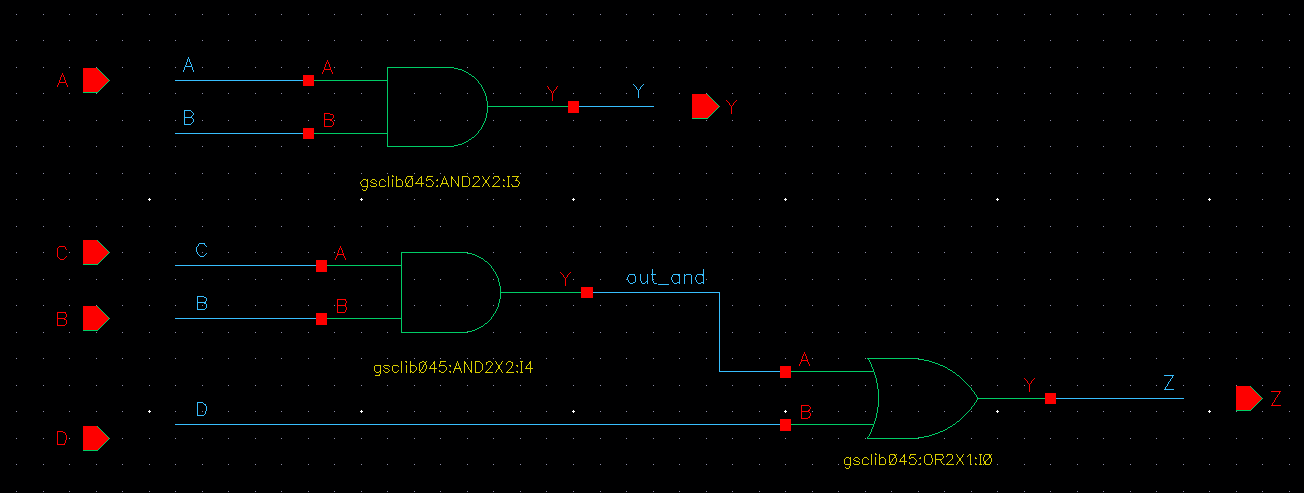
\includegraphics[width=0.72\linewidth]{assets/black_cell.png}
\caption{Black cell: produces both outputs -- $Y = A \cdot B$ (group
propagate) and $Z = (C \cdot B) + D$ (group generate) -- from two AND2X2
gates and one OR2X1.}
\end{figure}

\subsection{Registers}
All registers are built from per-bit \sig{DFFQX1} D flip-flops, clocked
synchronously off the shared \sig{CLK}.

\begin{figure}[htbp]
\centering
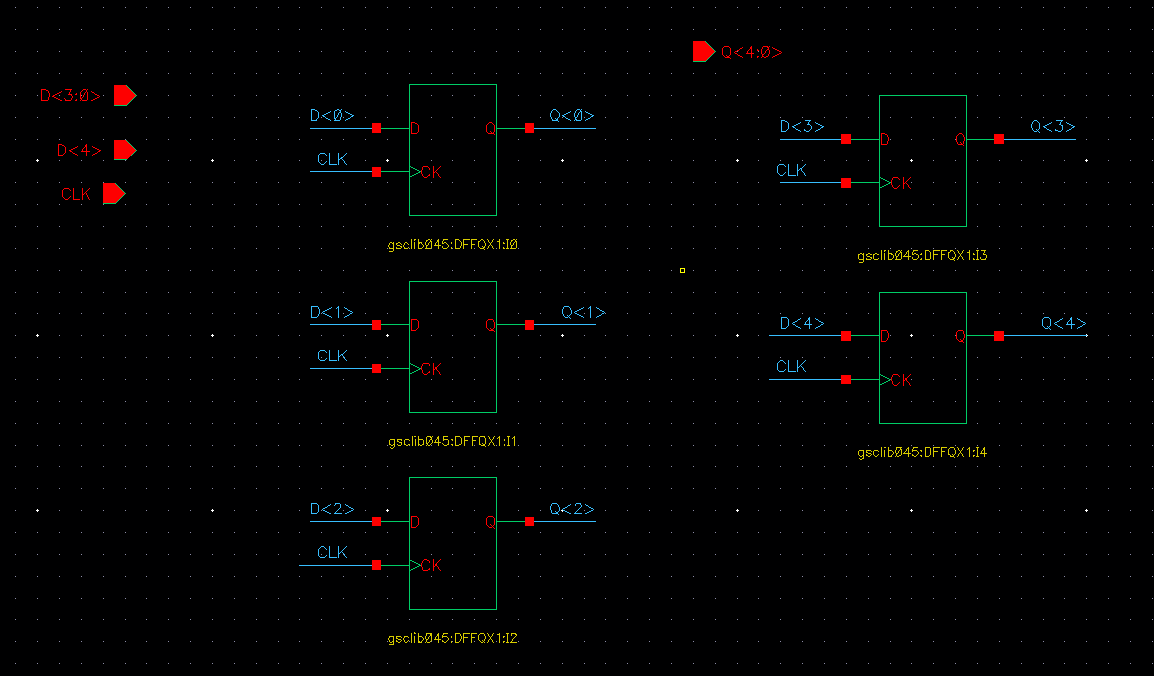
\includegraphics[width=0.62\linewidth]{assets/reg_4bit.png}
\caption{4-bit register -- one \sig{DFFQX1} per bit of $A$, $B$, or $C$.}
\end{figure}
\begin{figure}[htbp]
\centering
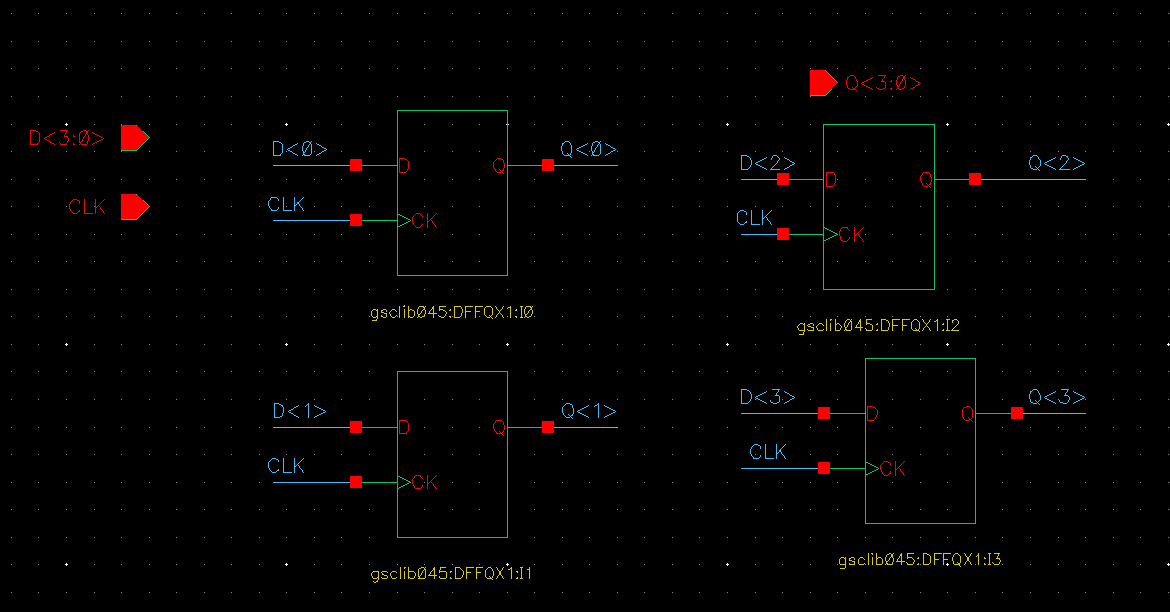
\includegraphics[width=0.62\linewidth]{assets/reg_5bit.png}
\caption{5-bit register -- latches the adder's output $X$.}
\end{figure}
\begin{figure}[htbp]
\centering
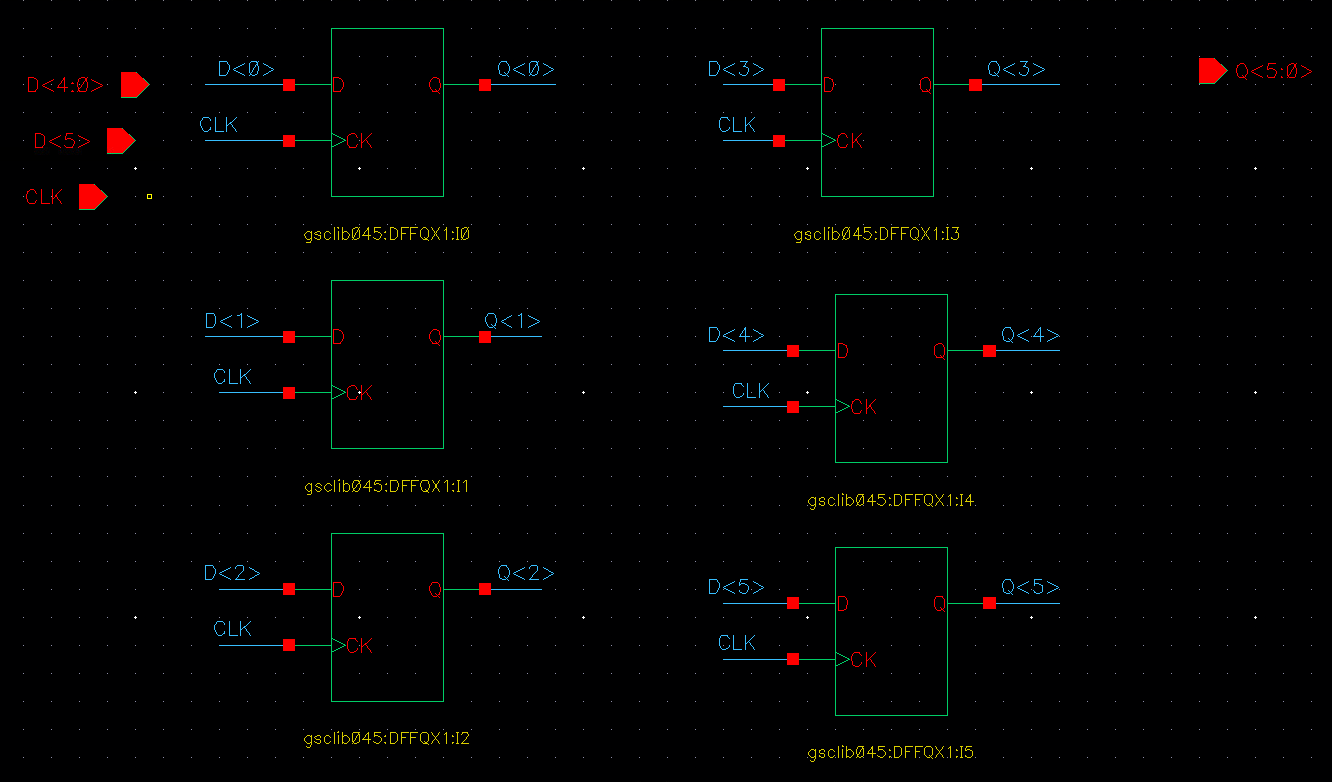
\includegraphics[width=0.75\linewidth]{assets/reg_6bit.png}
\caption{6-bit register -- latches the final ALU output $Y$.}
\end{figure}

Combining PG, Gray, and Black cells into a prefix tree lets the adder
compute every carry in parallel, avoiding the accumulating delay of a
ripple-carry chain.

%=====================================================================
\section{Physical Layout}
%=====================================================================
\emph{The physical layout below covers the adder only; the subtractor
reuses the same instantiated cells.}

\fig{adder_floorplan_redlines}{0.95}{Floor plan of the adder: two rows of
\sig{4bit\_adder\_pg} / \sig{4bit\_adder\_gray\_cell} / \sig{4bit\_adder\_black\_Cell}
cells, followed by the XOR2X1 sum-bit row.}

\fig{adder_layout_screenshot}{0.95}{Full adder layout in Virtuoso Layout Suite XL.}

\fig{layout_zoom1}{0.95}{Layout, zoomed in -- routing detail across the PG/Gray/Black cell boundary.}

\fig{layout_zoom2}{0.95}{Layout, zoomed in further -- metal and via detail on the standard-cell rows.}

\fig{layout_zoom3}{0.95}{Layout, zoomed in to transistor-level detail, showing the \sig{out\_gray} and \sig{out\_black} internal nets.}

%=====================================================================
\section{Verification: DRC \& LVS}
%=====================================================================

Design Rule Checking (DRC) verifies the physical integrity of the layout --
confirming that component placement and wire routing satisfy the
fabrication process's geometric rules (minimum spacing, width, enclosure,
etc.). Layout-Versus-Schematic (LVS) checking extracts the actual
transistor-level netlist from the layout and compares it against the
original schematic, confirming that every component and every pin
connection (the netlist) matches exactly. Both checks passed cleanly.

\fig{lvs_check}{0.92}{LVS run: schematic and layout netlists match, 0 errors.}
\fig{drc_check1}{0.92}{DRC run, screen 1/2: rule-check summary.}
\fig{drc_check2}{0.92}{DRC run, screen 2/2: ``Design Rule Check Finished Normally,'' 0 total DRC results.}

%=====================================================================
\section{Functional Verification}
%=====================================================================

\subsection{Adder}
The adder was verified first, in isolation, against a dedicated testbench.

\fig{adder_tb_schematic}{0.85}{Adder testbench: piecewise-linear sources drive $A$ and $B$; the adder's $S$ and $C\_OUT$ outputs are probed.}
\fig{adder_tb_waveform}{0.85}{Adder transient response: $C\_OUT$ and $C[3{:}0]$ track the expected sum of the stepped $A$ and $B$ inputs. (\sig{C} here is a convenience bus for the waveform display, not the ALU's actual carry-out signal.)}

\subsection{Subtractor}
\fig{subtractor_tb_schematic}{0.85}{Subtractor testbench.}
\fig{subtractor_tb_waveform}{0.85}{Subtractor transient response: $Y[4{:}0]$ tracks $X - C$ across the stepped test vectors.}

\subsection{Full ALU}
With the adder and subtractor independently verified, the complete ALU was
exercised end-to-end.

\fig{alu_tb_schematic}{0.92}{Full-ALU testbench: $A$, $B$, $C$ driven by independent piecewise-linear sources, clocked by a shared \sig{CLK}.}
\fig{alu_tb_waveform}{0.92}{Full-chip transient simulation across several clock cycles: $A$, $B$, $C$, the internal sum $X$, and the final result $Y$.}
\fig{alu_tb_waveform_zoom}{0.92}{Zoomed transient view of the same simulation.}

In the first clock cycle, $A$ and $B$ are latched into the adder. In the
second cycle, the partial sum appears as $X$ and is immediately fed into
the subtractor. In the third cycle, the subtraction result -- after having
$C$ subtracted -- appears at the output as $Y$.

\subsubsection{Overflow Boundary Check}
Finally, the design was pushed to its signed-range boundaries, exercising
both the largest and smallest representable results ($-23$ and $+22$):

\fig{overflow_check_annotated}{0.85}{Overflow boundary test. The three
annotated clock edges (translated from the original Hebrew) mark:
\textbf{1st edge} -- $A$ and $B$ are latched into their input registers;
\textbf{2nd edge} -- the partial sum is latched into register $X$;
\textbf{3rd edge} -- after subtracting $C$, the final result is latched
into $Y$.}

%=====================================================================
\section{Timing Analysis: Critical Path \& Voltage Impact}
\label{sec:timing}
%=====================================================================

\subsection{Critical Path Analysis}
To determine the maximum operating frequency, the critical (slowest)
register-to-register path must be identified. For any such path, the total
delay from one register's clock-to-Q output, through the intervening
combinational logic, to the next register's data input, must resolve
before that register's setup time expires:
\[
T_{cyc} > T_{pcq,launch} + T_{logic} + T_{setup,capture}
\]

Tracing the dataflow of Figure~\ref{fig:alu-dataflow}, there are four
register-to-register combinational paths:

\begin{enumerate}
  \item $A\text{-reg} \rightarrow \text{Adder} \rightarrow X\text{-reg}$
  \item $B\text{-reg} \rightarrow \text{Adder} \rightarrow X\text{-reg}$ \quad(structurally identical delay to path 1 -- symmetric adder inputs)
  \item $X\text{-reg} \rightarrow \text{Subtractor} \rightarrow Y\text{-reg}$
  \item $C\text{-reg} \rightarrow \text{Subtractor} \rightarrow Y\text{-reg}$
\end{enumerate}

Paths 1 and 2 share the same delay by construction, so only \textbf{three
distinct delay values} need to be characterized.

We need to determine, for each path: the combinational logic delay, the
flip-flop's clock-to-Q (\(t_{CQ}\)) delay, and the flip-flop's setup time.

\fig{alu_block_diagram_criticalpath}{0.85}{ALU dataflow, annotated with the register boundaries used for critical-path analysis.}

\subsection{Setup Time}
\label{sec:setup-time}
Setup time -- the minimum interval the data must be stable before the
clock's rising edge -- was measured directly in simulation, rather than
taken from a library value.

\fig{setup_tb_schematic}{0.85}{Setup-time testbench: a single \sig{DFFQX1}
driven by independent CLK and DATA sources, with the data edge given a
programmable negative delay relative to the clock.}

The clock was driven with continuous rising/falling edges, while the data
input received a single transition timed relative to it. By sweeping a
\emph{negative} delay on the data edge -- i.e.\ moving the data transition
earlier relative to the clock edge -- the point at which the flip-flop just
barely still captures correctly identifies the setup time exactly.

\fig{setup_timing_diagram}{0.55}{Definition of $T_{SETUP}$: the window
before the clock's rising edge during which data must remain stable. If the
output still transitions correctly, the setup requirement was met; if not,
the delay was insufficient.}

\textbf{At 1.2\,V:} the delay sweep ran coarsely from 0--200\,ps, then was
refined to 0--50\,ps, then further refined to 15--25\,ps in 10 steps.
Below $\sim$20\,ps the output became unstable; above it, the output
remained stable. \textbf{Setup time $\approx$ 20\,ps.}

\fig{setup_sweep_1p2v}{0.85}{Setup-time sweep at 1.2\,V: CLK, DATA, and the
family of $Q$ traces for each swept delay, converging on $\approx$20\,ps.}

\textbf{At 0.9\,V:} sweeping between $-30$ and $-50$\,ps (bisection-style),
the hold boundary was measured at \textbf{$\approx-44$\,ps}, i.e.\ a setup
time of $\approx$44\,ps.

\fig{setup_params_panel}{0.55}{The parametric sweep configuration used to
locate setup time: \sig{tsetup} swept via \sig{LinearStepCount} while the
output \sig{Q} family is inspected for the first stable transition (panel
captured with \sig{VDD}\,=\,1.2; \sig{VDD} was set to 0.9 separately for the
0.9\,V run below).}
\fig{setup_sweep_0p9v}{0.85}{Setup-time sweep at 0.9\,V ($V_{DD}=0.9$\,V): the boundary shifts to $\approx-44$\,ps as expected from the reduced drive strength.}

In practice, the total path delay is the combinational logic delay plus the
flip-flop's $t_{CQ}$ per stage, and in a hierarchical design this delay
\emph{accumulates} stage to stage -- each additional block adds its own
propagation delay on top of what came before. For the subtractor
specifically, the critical delay is bounded by the time it takes the
carry-out ($COUT$) to fully propagate and settle at the MSB.

\subsection{Combined Logic Delay + $t_{CQ}$}
\fig{subtractor_delay_schematic}{0.85}{Testbench for measuring the
combined $t_{CQ} + t_{sub,max}$ delay through the subtractor's $COUT$ path.}

\textbf{At 1.2\,V:}
\[
t_{cq} + t_{sub,max} = \tfrac{1}{2}\left(0.2029\,\mathrm{ns} + 0.2143\,\mathrm{ns}\right) = 0.209\,\mathrm{ns}
\]
\fig{cout_delay_1p2v}{0.85}{$COUT$ delay measurement at 1.2\,V: cursors at
30.2029\,ns and 50.2143\,ns bracket the 20\,ns clock half-period, giving
the 0.2029/0.2143\,ns delays averaged above.}

\textbf{At 0.9\,V:}
\fig{cout_delay_0p9v_b}{0.85}{$COUT$ delay measurement at 0.9\,V ($V_{DD}=900$\,mV
trace amplitude): cursors at 30.4431\,ns and 50.4453\,ns give the
0.4431/0.4453\,ns delays averaged below.}
\[
t_{cq} + t_{sub,max} = \tfrac{1}{2}\left(0.443\,\mathrm{ns} + 0.4453\,\mathrm{ns}\right) = 0.444\,\mathrm{ns}
\]

\subsection{Maximum Frequency}
\label{sec:fmax}

\textbf{At 1.2\,V:}
\[
T_{cyc} \ge T_{setup} + t_{cq} + t_{sub,max} = 20\,\mathrm{ps} + 0.209\,\mathrm{ns} = 0.229\,\mathrm{ns}
\ \Rightarrow\ f_{max} \approx 4.37\,\mathrm{GHz}
\]

\textbf{At 0.9\,V:}
\[
T_{cyc} \ge T_{setup} + t_{cq} + t_{sub,max} = 44\,\mathrm{ps} + 0.444\,\mathrm{ns} = 0.488\,\mathrm{ns}
\ \Rightarrow\ f_{max} \approx 2.05\,\mathrm{GHz}
\]

\begin{figure}[H]
\centering
\begin{tikzpicture}
\begin{axis}[
  width=0.8\linewidth, height=6.6cm,
  ybar stacked, bar width=36pt,
  ymin=0, ymax=570,
  ylabel={Cycle-time budget, $T_{cyc}$ (ps)},
  symbolic x coords={1.2 V, 0.9 V},
  xtick=data,
  enlarge x limits=0.32,
  axis lines*=left,
  ymajorgrids, grid style={gridline, line width=0.4pt},
  every axis plot/.append style={draw=none},
  legend style={at={(0.5,1.14)}, anchor=north, legend columns=-1, draw=none,
                font=\small, /tikz/column 2/.style={column sep=14pt}},
]
\addplot+[fill=accentblueLight] coordinates {(1.2 V,20) (0.9 V,44)};
\addplot+[fill=accentblue,
  nodes near coords, point meta=explicit symbolic,
  every node near coord/.style={font=\scriptsize\bfseries, text=white}]
  coordinates {(1.2 V,209) [209 ps] (0.9 V,444) [444 ps]};
\legend{Setup time, Logic delay $+\,t_{CQ}$}
\node[font=\scriptsize\bfseries, color=accentblue, anchor=west] at (axis cs:1.2 V,20) [xshift=22pt] {20\,ps};
\node[font=\scriptsize\bfseries, color=accentblue, anchor=west] at (axis cs:0.9 V,44) [xshift=22pt] {44\,ps};
\node[font=\bfseries\large, color=accentorange] at (axis cs:1.2 V,340) {4.37 GHz};
\node[font=\scriptsize, color=inksecondary] at (axis cs:1.2 V,295) {$T_{cyc}=229$\,ps};
\node[font=\bfseries\large, color=accentorange] at (axis cs:0.9 V,540) {2.05 GHz};
\node[font=\scriptsize, color=inksecondary] at (axis cs:0.9 V,495) {$T_{cyc}=488$\,ps};
\end{axis}
\end{tikzpicture}
\caption{Cycle-time budget at each corner: each bar is literally
$T_{cyc} = T_{setup} + (t_{cq}+t_{sub,max})$, stacked to show where the
time actually goes, with the resulting $f_{max} = 1/T_{cyc}$ called out
above. Both components grow at the lower supply -- not just the logic
delay -- because reduced drive current slows the flip-flops themselves too
(see \S\ref{sec:part2-q45} and the $t = C\Delta V / I_{AVG}$ relation
below); that combined growth is what nearly doubles the cycle time and
roughly halves $f_{max}$ at 0.9\,V.}
\label{fig:fmax-vdd}
\end{figure}

We can explain this trend with the familiar delay relation
\[
t = \frac{C \cdot \Delta V}{I_{AVG}}
\]
lower $V_{DD}$ reduces the average drive current $I_{AVG}$ available to
charge/discharge the same node capacitance $C$, which lengthens every gate
delay and pulls $f_{max}$ down.

\fig{alu_full_sim_4p33ghz}{0.92}{Full ALU simulated at 1.2\,V near $f_{max}$ (4.33\,GHz target, $T_{cyc}=0.21$\,ns; the corrected $f_{max}$ from \S\ref{sec:fmax} is 4.37\,GHz): $A$, $B$, $X$, $C$, and $Y$ tracking correctly cycle-to-cycle.}

\subsection{Rise / Fall Times}
Rise time (10\%--90\%) and fall time (90\%--10\%) were measured for every
signal at both corners, using \sig{riseTime(VT(SIGNAL) 0 nil <VDD> nil 10 90 nil "time")}
and the equivalent \sig{fallTime(...)} call.

\begin{table}[H]
\centering
\begin{tabular}{@{}lcc@{}}
\toprule
\rowcolor{accentblue!10}
\textbf{Signal} & \textbf{Rise time, 1.2\,V} & \textbf{Rise time, 0.9\,V} \\
\midrule
$A[3{:}0]$, $B[3{:}0]$, $C[3{:}0]$ & $<$8\,fs & $<$8\,fs \\
CLK & 8\,fs & 8\,fs \\
$A$\,$Q$ (out of 4-bit reg) & $<$10.98\,ps & $<$17.48\,ps \\
$B$\,$Q$ (out of 4-bit reg) & $<$13.35\,ps & $<$20.83\,ps \\
$C$\,$Q$ (out of 4-bit reg) & $<$15.46\,ps & $<$23.21\,ps \\
Adder sum $S[3{:}0]$ & $<$10.84\,ps & $<$19.07\,ps \\
Adder $C_{OUT}$ & 10.87\,ps & 18.88\,ps \\
$X[4{:}0]$ & $<$18.92\,ps & $<$31.08\,ps \\
Sub. result $Y[4{:}0]$ & $<$10.87\,ps & $<$18.99\,ps \\
Sub. $C_{OUT}$ & 10.67\,ps & 19.01\,ps \\
$Y[5{:}0]$ & $<$14.48\,ps & $<$24.73\,ps \\
\bottomrule
\end{tabular}
\caption{Rise times, both corners -- every signal clears the 50\,ps requirement with wide margin.}
\end{table}

\begin{table}[H]
\centering
\begin{tabular}{@{}lcc@{}}
\toprule
\rowcolor{accentblue!10}
\textbf{Signal} & \textbf{Fall time, 1.2\,V} & \textbf{Fall time, 0.9\,V} \\
\midrule
$A[3{:}0]$, $B[3{:}0]$, $C[3{:}0]$ & $<$8\,fs & $<$8\,fs \\
CLK & 8\,fs & 8\,fs \\
$A$\,$Q$ (out of 4-bit reg) & $<$10.98\,ps & $<$17.48\,ps \\
$B$\,$Q$ (out of 4-bit reg) & $<$13.35\,ps & $<$20.83\,ps \\
$C$\,$Q$ (out of 4-bit reg) & $<$15.54\,ps & $<$23.21\,ps \\
Adder sum $S[3{:}0]$ & $<$10.84\,ps & $<$19.07\,ps \\
Adder $C_{OUT}$ & 10.87\,ps & 18.88\,ps \\
$X[4{:}0]$ & $<$19.00\,ps & $<$31.07\,ps \\
Sub. result $Y[4{:}0]$ & $<$10.89\,ps & $<$18.99\,ps \\
Sub. $C_{OUT}$ & 10.67\,ps & 19.01\,ps \\
$Y[5{:}0]$ & $<$14.48\,ps & $<$24.73\,ps \\
\bottomrule
\end{tabular}
\caption{Fall times, both corners -- likewise all clear the 50\,ps requirement.}
\end{table}

%=====================================================================
\section{Part 2: Clock Generation -- Ring Oscillator}
\label{sec:part2}
%=====================================================================

\emph{This section answers a numbered set of questions from the assignment
sheet (Q4--Q7); the numbering is preserved from the original assignment
rather than restarted at 1, so the answers stay traceable to the source
questions.}

\paragraph{Q4 -- Inverter sizing vs.\ frequency.}
\label{sec:part2-q45}
Increasing the size of the ring's inverters increased the oscillation
frequency $f_{osc}$. A larger inverter has more drive strength, which
reduces its propagation delay $t_d$; since $t_d$ and $f_{osc}$ are
inversely related, a shorter per-stage delay raises the frequency.
Larger inverters also drive larger capacitive loads without the delay
penalty a smaller inverter would incur under the same load.

\paragraph{Q5 -- Adding RC chains.}
Adding RC chains between stages \emph{decreased} $f_{osc}$: the added
series resistance and shunt capacitance increase each stage's time delay,
since the inverters now have to charge/discharge a larger effective load.

\paragraph{Q6 -- Five-inverter ring, resistance-tuned.}
The oscillator was built from 5 \sig{INXV1} inverters, with the tuning
resistance adjusted until the target frequency was reached.

\fig{ring_osc_ring_schematic}{0.85}{Five-stage \sig{INXV1} ring oscillator: each stage is an inverter followed by a tunable series resistor and shunt capacitor to ground.}
\fig{ring_osc_testbench_supply}{0.55}{Oscillator testbench: DC supply rails and the output load capacitor.}

With more inverter stages in the ring, the frequency was noticeably easier
to control without resorting to large resistor values.

\paragraph{Q7a -- Adding an output capacitor.}
Adding a capacitor at the output decreased the frequency, consistent with
the same load-vs-delay relationship: $f_{osc} = 2.5\,\mathrm{MHz}$ without
the load, dropping to $f_{osc} = 2.46\,\mathrm{MHz}$ once the capacitor was
added.

\fig{ring_osc_q7a_result}{0.85}{ADE Explorer result with the output capacitor added ($R=46.08$\,k$\Omega$, $C=1$\,pF): $f_{osc} = 2.463$\,MHz, matching the $\approx$2.46\,MHz reported above.}

\paragraph{Q7b -- Signal integrity impact.}
With the added capacitor, the rail-to-rail swing narrowed -- the output no
longer reached the full $0$--$1.2$\,V range -- and the rising/falling edges
softened. The \sig{INXV1} inverters simply weren't strong enough to drive
the larger capacitive load cleanly.

\paragraph{Q7c -- Switching to INXV2.}
Replacing the inverters with the larger \sig{INXV2} cell restored full
rail-to-rail swing and sharp edges -- in fact slightly better than the
original no-load case -- and \emph{increased} $f_{osc}$ above the loaded
\sig{INXV1} result, since the larger cell's higher drive strength reduced
per-stage delay despite the added load.

\fig{ring_osc_inxv2_result}{0.85}{ADE Explorer result after switching to \sig{INXV2}: full swing restored, $f_{osc} = 2.568$\,MHz.}

\begin{figure}[H]
\centering
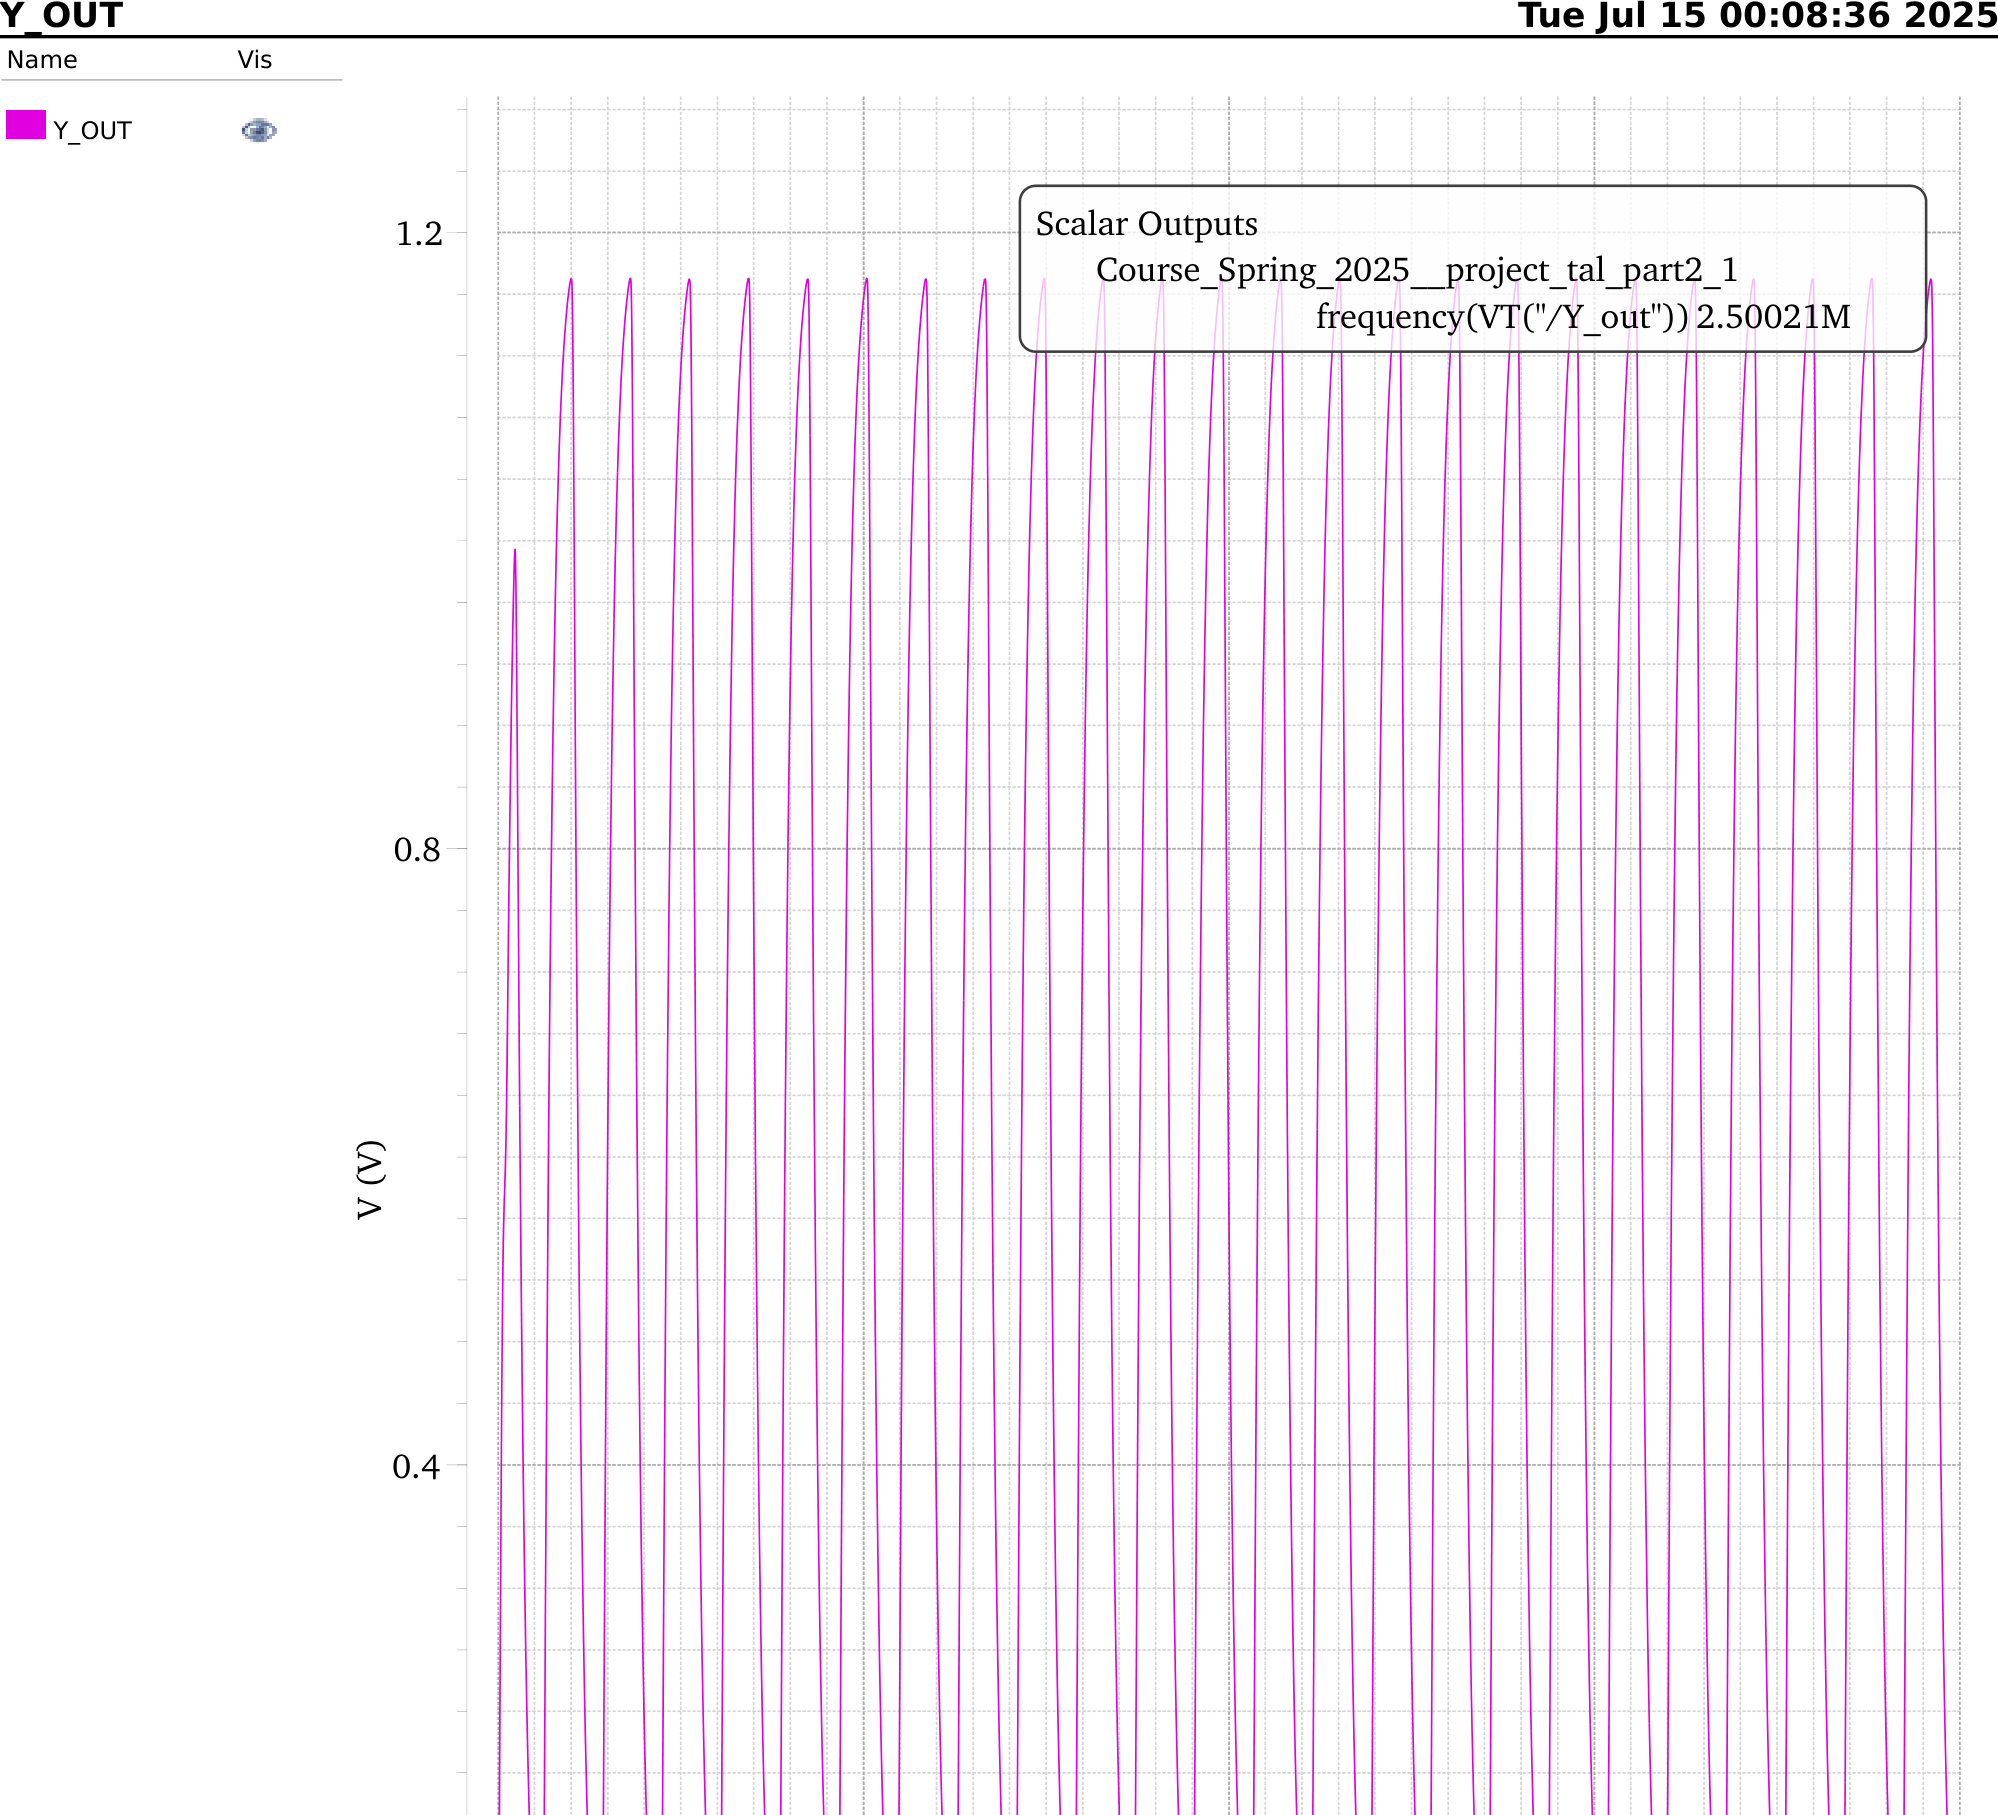
\includegraphics[width=0.85\linewidth]{assets/p34_yout_plot.png}
\caption{$Y_{OUT}$ transient waveform, baseline \sig{INXV1} ring with no output load: $f_{osc} = 2.50021$\,MHz.}
\end{figure}

\begin{figure}[H]
\centering
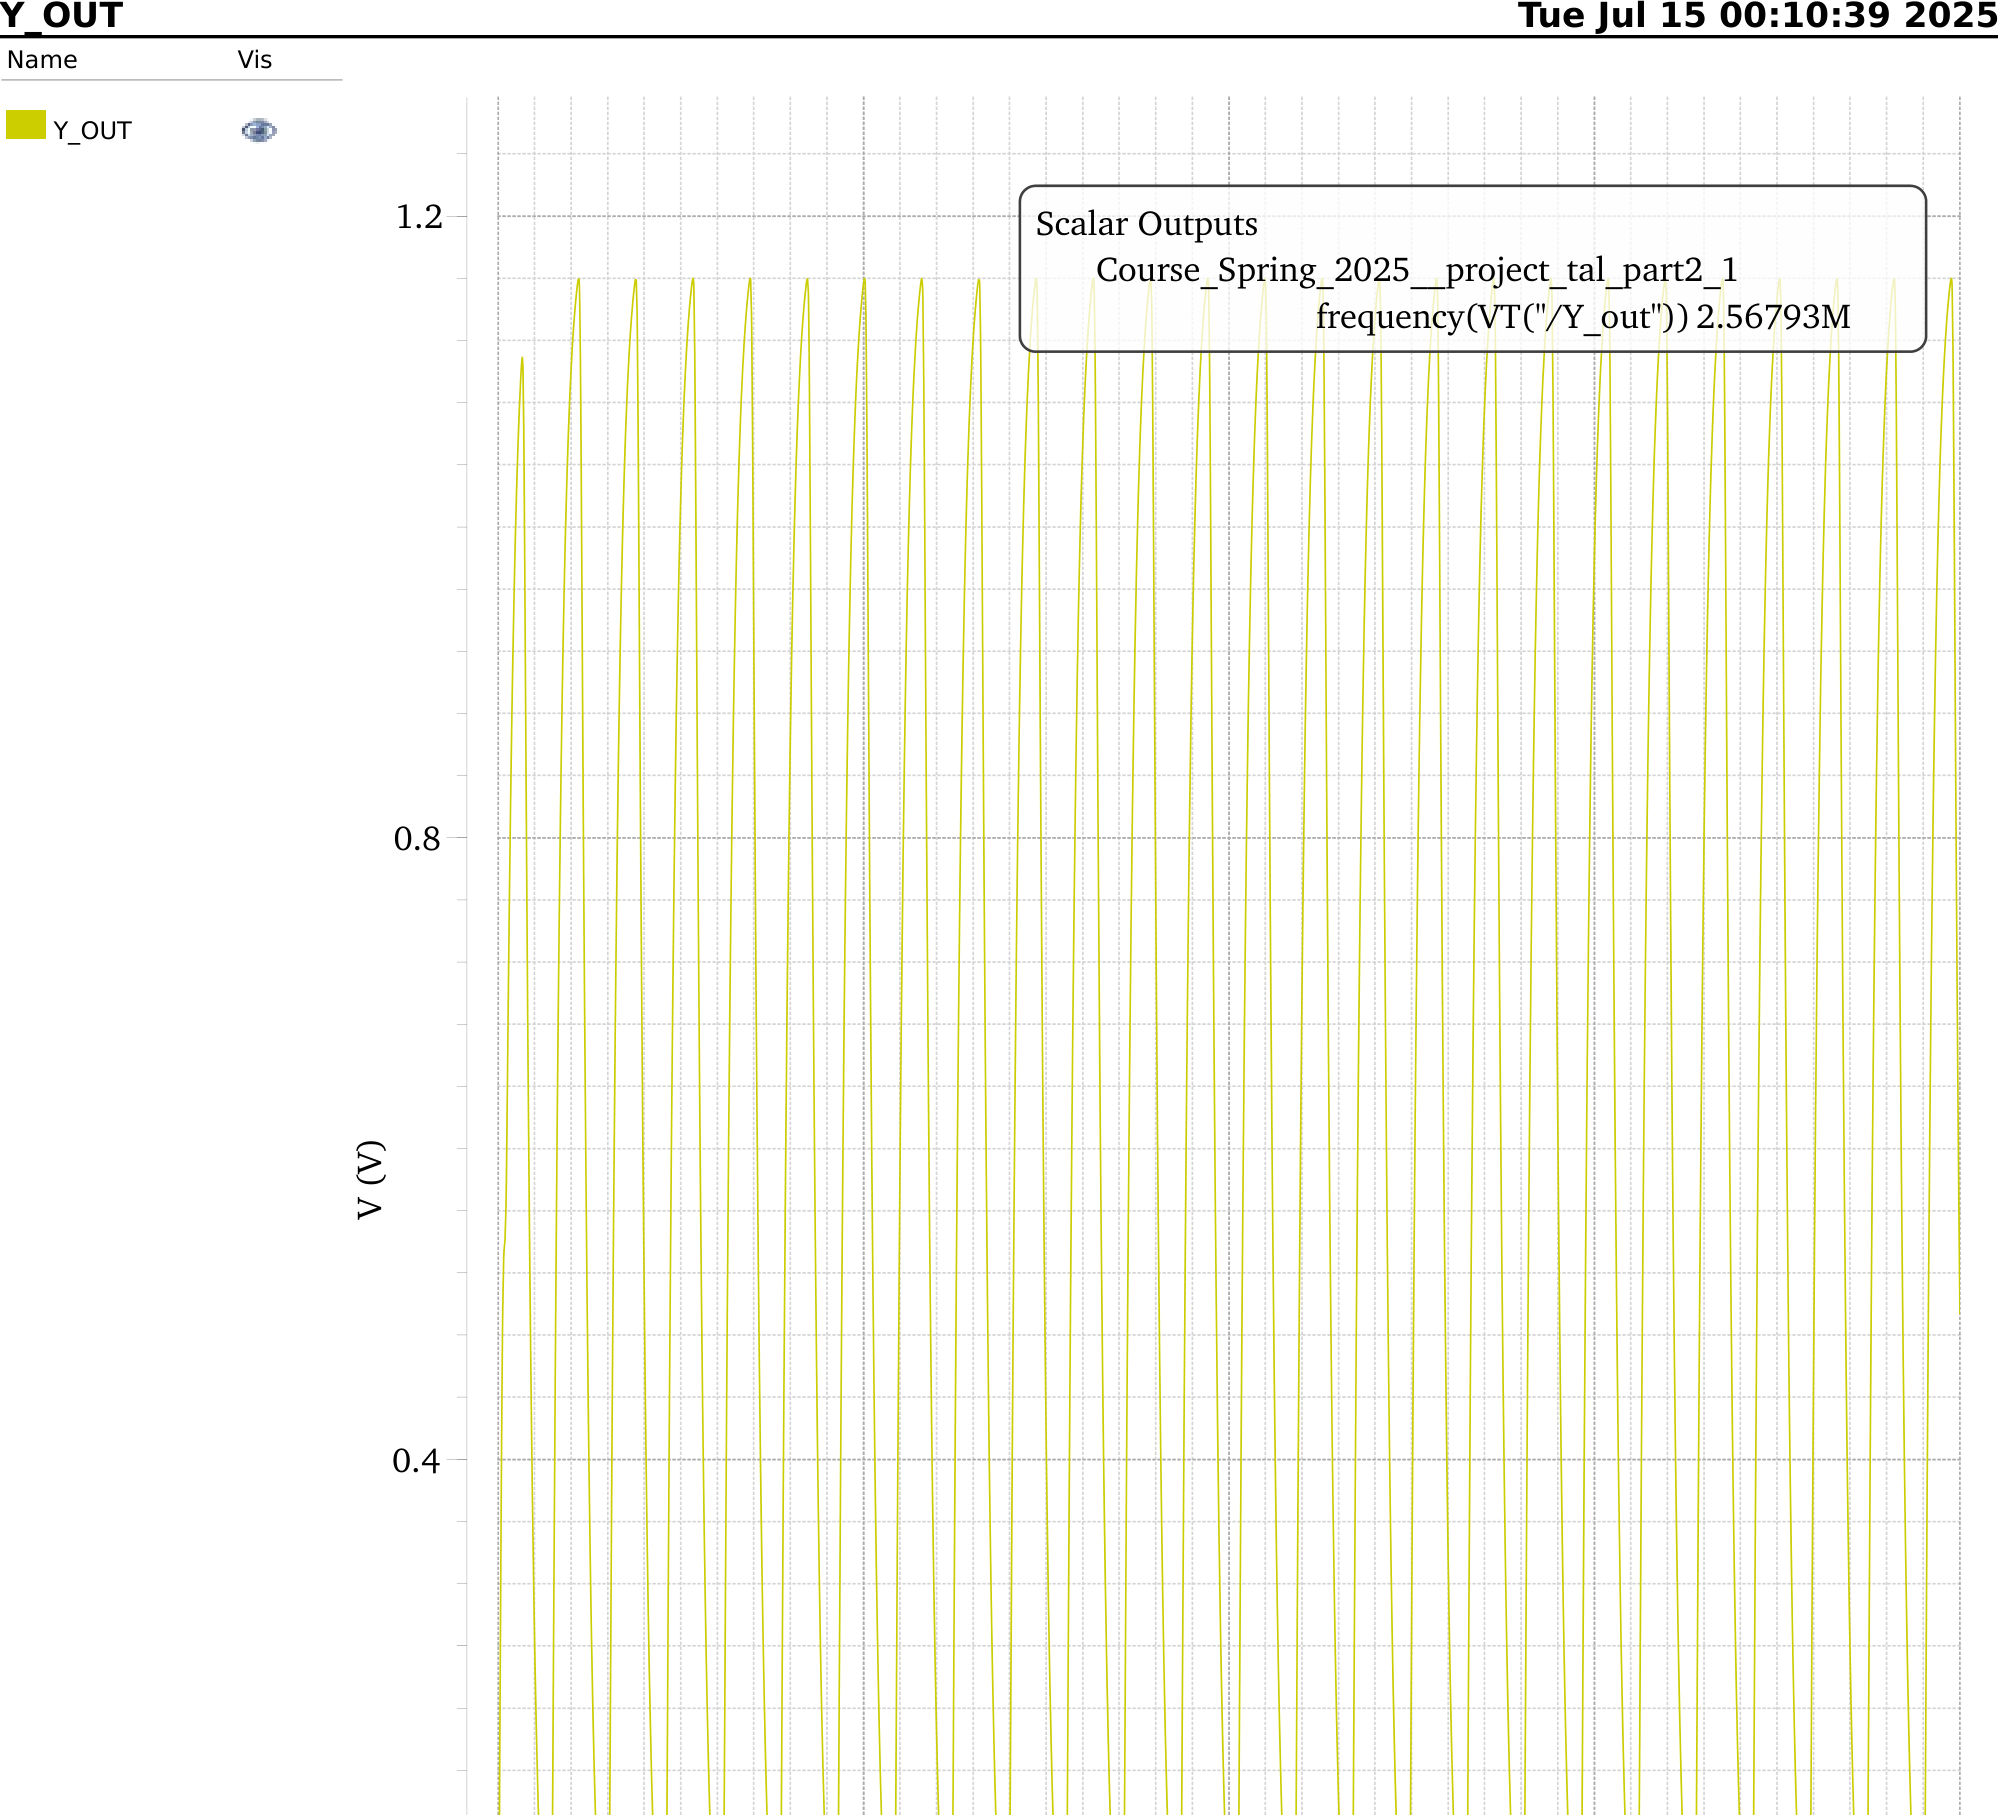
\includegraphics[width=0.85\linewidth]{assets/p35_yout_plot.png}
\caption{$Y_{OUT}$ transient waveform after switching to \sig{INXV2} with the output capacitor present: $f_{osc} = 2.56793$\,MHz -- higher than the loaded \sig{INXV1} case, confirming Q7c.}
\end{figure}

%=====================================================================
\section{Conclusion}
%=====================================================================

The ALU meets its functional specification -- \sig{ADD} and \sig{SUB} both
verified against dedicated testbenches, with the full datapath additionally
exercised end-to-end including its signed-overflow boundaries -- and its
physical implementation is signoff-clean (DRC and LVS both pass with zero
violations). The Sklansky adder's parallel-prefix structure delivers a
measured $f_{max}$ of \textbf{4.37\,GHz at 1.2\,V}, degrading to
\textbf{2.05\,GHz at 0.9\,V} as reduced drive current lengthens
every stage's propagation delay -- the same physical mechanism explored
independently in the Part 2 ring-oscillator study, where inverter sizing
and output loading traded off against $f_{osc}$ in exactly the same
direction. Together, the two parts demonstrate the same design
principle from opposite ends: drive strength buys speed, and every
picosecond of that budget has to be accounted for, from a single inverter
stage up to a full datapath's critical path.

\end{document}
